\documentclass[12pt]{report}

% 古い環境でエラーになる場合は,以下で置き換える
%\documentclass[12pt,report]{ltjsbook}

% This template must be compiled by lualatex.
% TeXStudio automatically select the compiler by the next line.
% !TeX program = lualatex

%%%%%%%%%%%%%%%%%%%%%%%%%%%%%%%%%%%%%%%%%%%%%%%%%%%%%%%%%%%%%%%%%%%%%%%%%%%
%% preamble for specifying packages 
\label{pre:package}
\usepackage{ifpdf}
\usepackage{fullpage}
%\usepackage{tocbibind} % to show "参考文献" in TOC
%\usepackage[title,titletoc]{appendix}
\usepackage{indentfirst}
\usepackage{graphicx,color}
\usepackage{setspace}
\usepackage{amssymb}
\usepackage{amsmath}
%\usepackage{slashbox}
%\usepackage{multirow}
\usepackage{xspace}
\usepackage{ifthen}
\usepackage{algorithm}
\usepackage{algorithmic}

\usepackage[pdfencoding=auto]{hyperref}
\hypersetup{%
	bookmarks=true,%
	bookmarksdepth=subsubsection,%
	bookmarksnumbered=true,%
	bookmarkstype=toc,%
	pagebackref=true,%
	linktocpage=true,%
	pdftitle={Bachelor/Master/Ph.D. Thesis},%
	pdfauthor={Author},%
	pdfkeywords={Key words},%
	linkcolor=blue,%
	anchorcolor=blue,%
	urlcolor=blue%
}
	
%%%%%%%%%%%%%%%%%%%%%%%%%%%%%%%%%%%%%%%%%%%%%%%%%%%%%%%%%%%%%%%%%%%%%%%%%%%
%% preamble for specifying packages 
\label{pre:command}
% Reference
\newcommand{\Cemb}[1]{\phantomsection \addcontentsline{toc}{chapter}{#1}\chapter*{#1}}
\newcommand{\tref}[1]{表~\ref{#1}}
\newcommand{\eref}[1]{式~(\ref{#1})}
\newcommand{\fref}[1]{図~\ref{#1}}
\newcommand{\alref}[1]{アルゴリズム~\ref{#1}}
\newcommand{\sref}[1]{\ref{#1}章}
\newcommand{\cref}[1]{\ref{#1}章}
\newcommand{\appref}[1]{付録~\ref{#1}}
% Equation
\newcommand{\argmax}{\mathop{\rm argmax}\limits}
\newcommand{\argmin}{\mathop{\rm argmin}\limits}
\newcommand{\norm}[2]{\left|\left|#1\right|\right|^{#2}}
\renewcommand{\bibname}{参考文献}
%
\newcommand{\degree}[1]{
	\vspace*{45mm}
	{\huge 2016年度~~#1論文}
	\\
}
\renewcommand{\title}[1]{
	\vspace{15mm}
	{\huge \bfseries #1 }
	\\
}
\newcommand{\supervisor}[1]{
	\vspace{75mm}
	{\Large 指導教員~~~ #1}
	\\
}
\newcommand{\study}{
	\vspace{10mm}
	{\Large 研究指導名~~~コンピュータービジョン研究}
	\\
}
\newcommand{\affiliation}[1]{
	\vspace{10mm}
	{\Large #1}
	\\
}
\renewcommand{\author}[2]{
	{\Large
	#2~~#1
	}
	\\
}
\renewcommand{\date}{
	\vspace{10mm}
	{\Large  2016年 2月 6日~~提出}
}


\makeatletter
\DeclareRobustCommand\onedot{\futurelet\@let@token\@onedot}
\def\@onedot{\ifx\@let@token.\else.\null\fi\xspace}
\def\eg{\emph{e.g}\onedot} \def\Eg{\emph{E.g}\onedot}
\def\ie{\emph{i.e}\onedot} \def\Ie{\emph{I.e}\onedot}
\def\cf{\emph{c.f}\onedot} \def\Cf{\emph{C.f}\onedot}
\def\etc{\emph{etc}\onedot} \def\vs{\emph{vs}\onedot}
\def\wrt{w.r.t\onedot} \def\dof{d.o.f\onedot}
\def\etal{et~al\onedot}
\def\vice{\emph{vice versa}}
\makeatother

\onehalfspacing


% 添削時に有効にする
%\doublespacing

\begin{document}
%%%%%%%%%%%%%%%%%%%%%%%%%%%%%%%%%%%%%%%%%%%%%%%%%%%%%%%%%%%%%%%%%%%%%%%%%%%
%% header
\pagenumbering{roman}

\hypersetup{pageanchor=false}
	%% Title page
	\begin{titlepage}
\begin{center}

	\degree{Master} % type of degree
	\title{Anime Faces Generation Corresponding to Human Faces with Finetuned Gnenerator} % thesis tytle
	\supervisor{Prof. Hiroshi Ishikawa} % Name of thesis adviser
	\study
	\affiliation{Waseda Univ., Fundamental Science and Engineering, Computer Science}
	\author{Wang Yiwen}{5120FG52}
	\date

\end{center}
\clearpage\thispagestyle{empty}
\end{titlepage}

\hypersetup{pageanchor=true}
\thispagestyle{plain}
%% Abstract
\Cemb{論文概要}
This document is a template of bachelor, master, or Ph.D. thesis.

\par
Abstract is here.
Maybe it's better to write abstract at the end of your thesis writing.

\clearpage
%% Acknowledgements
\Cemb{謝辞}
Let's thank people who somehow contribute to complete your thesis work here.

\begin{flushright}
\par
\noindent
\today

\par
\noindent
Author name
\end{flushright}
%\clearpage\thispagestyle{empty}

\clearpage
%% Table of Contents
\tableofcontents
\listoffigures
\listoftables
%\listofalgorithms
%\addcontentsline{toc}{chapter}{List of Algorithms}
\clearpage

%%%%%%%%%%%%%%%%%%%%%%%%%%%%%%%%%%%%%%%%%%%%%%%%%%%%%%%%%%%%%%%%%%%%%%%%%%%
%% main body
\pagenumbering{arabic}

%% Introduction
\chapter{Introduction}
\label{ch:intro}
This chapter shows some examples of \LaTeX{} writing.

\section{Equations}
There are several commands to write equations such as \textbackslash{}equation, \textbackslash{}eqnarray, and \textbackslash{}align.
This section shows examples of \textbackslash{}align as
\begin{align}
y = Ax+b.
\label{eq:exampleSingle}
\end{align}
You can refer any equation by using \textbackslash{}ref command as 式~\ref{eq:exampleSingle}.
This thesis template defines a useful command \textbackslash{}eref \eref{eq:exampleSingle}.

\par
\textbackslash{}align can shows multiple equations as
\begin{align}
y &= Ax+b ,
\label{eq:exampleMultiple1} \\
x &= K[R|t]X.
\label{eq:exampleMultiple2}
\end{align}
It is possible to assign a label to each equation as \eref{eq:exampleMultiple1} and \eref{eq:exampleMultiple2}.

\par
Matrix can be written by \textbackslash{}matrix commands.
When you need bracket (or parenthesis), you can use \textbackslash{}bmatrix (or \textbackslash{}pmatrix) as
\eref{eq:exampleMatrix}
\begin{align}
  P = 
	\begin{bmatrix}
		p_{11} & p_{12} & p_{13} & p_{14} \\
		p_{21} & p_{22} & p_{23} & p_{24} \\
		p_{31} & p_{32} & p_{33} & p_{34} 
	\end{bmatrix}.
\label{eq:exampleMatrix}
\end{align}

\section{Figures}
Here's an example how to put a figure.
Each figure should have a caption, which explains the contents of the figure, below the figure.
The size of a figure is adjustable by specifying its size.
In this example, the size is set as the width of the figure equals 60\% of column width. 
Same as equations, you can refer any figure by using \textbackslash{}ref command as 図~\ref{fig:example}.
This thesis template defines a useful command \textbackslash{}fref as \fref{fig:example}.
\begin{figure}[tb]
	\centering
		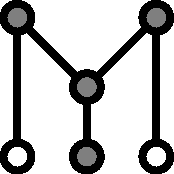
\includegraphics[width=0.6\hsize]{example-figure}
		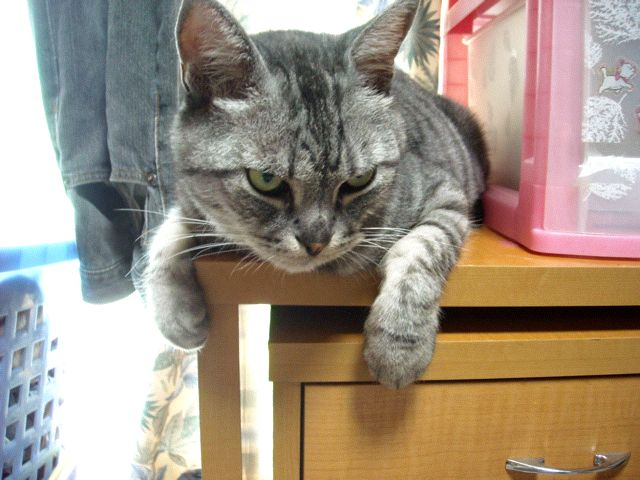
\includegraphics[width=0.6\hsize]{cat}
	\caption{Example of figure}
	\label{fig:example}
\end{figure}

\section{Tables}
Here's an example how to put a table.
Again, you can refer any table by using \textbackslash{}ref command as Table~\ref{tab:example}.
This thesis template defines a useful command \textbackslash{}tref as \tref{tab:example}.
More complicated table is shown in \tref{tab:example2}.
\begin{table}[tb]
	\centering
		\caption{Example of table}
		\begin{tabular}{r|c|c}
			\hline
			name & id & size \\
			\hline \hline
			John Doe & 1 & 100 \\
			Jane Doe & 3 & 150 \\
			\hline
		\end{tabular}
	\label{tab:example}
\end{table}
\begin{table}[tb]
\begin{center}
\caption{Exmple of complicated table}
\begin{tabular}{l|cc|cc||cc|cc||cc|cc}
\hline\hline
& \multicolumn{4}{c||}{pretest} & \multicolumn{4}{c||}{posttest} & \multicolumn{4}{c}{Gain} \\
\cline{2-13}
& \multicolumn{2}{c|}{Score} & \multicolumn{2}{c||}{Time} & \multicolumn{2}{c|}{Score} & \multicolumn{2}{c||}{Time} & \multicolumn{2}{c|}{Score} & \multicolumn{2}{c}{Time} \\
\hline
Group     & A     & P     & A    & P  & A     & P     & A    & P  & A     & P     & A    & P \\
\hline
Mean      & 18.48 & 14.59 & 5.25 & 5.28 & 28.52 & 21.89 & 3.95 & 4.28 & 10.04 & 7.30 & 1.30 & 1.12 \\
Std. dev. & 10.93 & 11.52 & 1.44 & 1.23 &  5.63 &  9.92 & 1.17 & 1.16 &  8.85 & 7.85 & 1.12 & 1.15 \\
\hline
p & \multicolumn{2}{c|}{0.21} & \multicolumn{2}{c||}{0.89} & \multicolumn{2}{c|}{0.00} & \multicolumn{2}{c||}{0.32} & \multicolumn{2}{c|}{0.23} & \multicolumn{2}{c}{0.22} \\
\hline\hline
\end{tabular}
\label{tab:example2}
\end{center}
\end{table}

\section{Algorithms}
Here's an example how to put an algorithm.
Same as figure, you can refer any table by using \textbackslash{}ref command as Algorithm~\ref{alg:example}.
This thesis template defines a useful command \textbackslash{}aref as \alref{alg:example}.
\alref{alg:example2} shows another type of algorithm which contains normal text.
See \href{http://en.wikibooks.org/wiki/LaTeX/Algorithms}{here} for more detail about algorithm, algorithmicx, and algorithm2e packages.
\begin{algorithm}
	 \caption{Example of algorithm copied from \href{http://www.math-linux.com/latex-26/faq/latex-faq/How-to-write-algorithm-and}{here}}
	\label{alg:example}
	\begin{algorithmic}
		\REQUIRE $n \geq 0 \vee x \neq 0$
		\ENSURE $y = x^n$
		\STATE $y \leftarrow 1$
		\IF{$n < 0$}
			\STATE $X \leftarrow 1 / x$
			\STATE $N \leftarrow -n$
		\ELSE
			\STATE $X \leftarrow x$
			\STATE $N \leftarrow n$
		\ENDIF
		\WHILE{$N \neq 0$}
			\IF{$N$ is even}
				\STATE $X \leftarrow X \times X$
				\STATE $N \leftarrow N / 2$
			\ELSE[$N$ is odd]
				\STATE $y \leftarrow y \times X$
				\STATE $N \leftarrow N - 1$
			\ENDIF
		\ENDWHILE
	\end{algorithmic}
\end{algorithm}

\begin{algorithm}
	\caption{Example of algorithm with text copied from \href{ftp://ftp.u-aizu.ac.jp/pub/tex/CTAN/macros/latex/contrib/algorithms/algorithms.pdf}{here}}
	\label{alg:example2}
	\begin{algorithmic}
		\IF{some condition is true}
		\STATE do some processing
		\ELSIF{some other condition is true}
		\STATE do some different processing
		\ELSIF{some even more bizarre condition is met}
		\STATE do something else
		\ELSE
		\STATE do
		\ENDIF
	\end{algorithmic}
\end{algorithm}


\section{Reference}
Citation can be done by \textbackslash{}cite command as \cite{Adamowicz92} and \cite{AlloucheSh92,BartonFi72a,CaludeP83}.
For citation, it is highly recommended to use BibTeX.
For more flexible bibliography, you can use \href{http://www.ctan.org/pkg/natbib}{natbib}.



\clearpage

%% Related works
\chapter{Literature Review}
\label{ch:literature}
Literature review is here.
It is required but not enough to explain related works.
Literature review needs to compare/cluster 
It is highly recommended to cluster related works based on your context.
\clearpage

%% Proposed method
\chapter{Proposed Method}
\label{ch:method}
Please don't start describing the detail of your proposed method at the beginning of this chapter.
You must control the level of detail of the description.
It is highly recommended to explain an overview of the proposed method, which corresponds to the coarsest information of the proposed method, at the first paragraph of the method description chapter.
It is great that you pur some figures for explaining overview.

\section{Detail of the proposed method}
\clearpage

%% Experimental results
\chapter{Experimental Results}
\label{ch:result}
Same as \cref{ch:method}, you must control the level of detail of the description.
It is highly recommended to explain an overview of the experiments.

\par
Each section must contain only one experiment, otherwise your sections may fail to tell readers wrong messages.
Each experiment must clarify the following components.
\begin{enumerate}
	\item purpose
	\item procedure accomplishing the purpose
	\item results obtained by performing the procedure
	\item consideration by comparing the expected results and the obtained results
\end{enumerate}

\section{Experiment A}

\subsection{Purpose}

\subsection{Procedure}

\subsection{Results}

\subsection{Consideration}
\clearpage

%% Conclusion
\chapter{Conclusion}
\label{ch:conclusion}
Conslusion is here
\clearpage

% 日本語を含む文献では, jplain, jabbrv などを指定し,
% pbibtex または upbibtex で処理すること.
\bibliographystyle{jplain}
%\bibliographystyle{tieice}  % 電子情報通信学会
%\bibliographystyle{tipsj}   % 情報処理学会
\bibliography{test,gc_ja}
\clearpage

%% Appendix
\appendix
% \addappheadtotoc

\chapter{Detail of implementation}
\label{apdx:implementation}
Let's wrote the detail of method implementation.
You can write the following information of softwares and libraries used for the implementation.
\begin{itemize}
	\item Name
	\item URL
	\item Version
	\item Any tips for installation/compilation
\end{itemize}
\clearpage

\chapter{Basic theory of A}
\label{apdx:A}
Appendices are supposed to be supplemental material of your thesis.
You can write the following components here.
\begin{itemize}
	\item Detail of implementation (softwares, libraries, etc.)
	\item Any data that does not well-fit into the main body of the thesis such as tables, figures, etc..
	\item Mathematical proof.
	\item Questionnaires for qualitative evaluations.
\end{itemize}
\clearpage

\end{document}
